%\documentclass[a0,landscape,posterdraft]{a0poster}
%\documentclass[a0b,landscape,final]{a0poster}
\documentclass[a0b,portrait,final]{a0poster}
\usepackage{colordvi,amsmath,epsfig,float,color,multicol,subfigure}
%\usepackage{grffile}
\usepackage[table]{xcolor}
\usepackage{pstricks,pst-node}
%\usepackage{txfonts}
\usepackage{tabularx}
\usepackage[framemethod=TikZ]{mdframed}
\usepackage{lipsum}

% landscape
% portrait
% a0b   ``DIN A0 big''. 915.1* 1200 mm 
% a0    ``DIN A0''.    839.6 * 1188.2 mm
% draft                 Gj�r om til A4 for testutskrift.
% final                 Gj�r at PS-fila blir i spesifisert st�rrelse;
%                       standard.
% ISO A0 size, 841 mm by 1189 mm.
% \tiny            12pt
% \scriptsize      14.4pt
% \footnotesize    17.28pt
% \small           20.74pt
% \normalsize      24.88pt
% \large           29.86pt
% \Large           35.83pt
% \LARGE           43pt
% \huge            51.6pt
% \Huge            61.92pt
% \veryHuge        74.3pt
% \VeryHuge        89.16pt
% \VERYHuge        107pt

% N�r du har kj�rt latex 'filnavn.tex', vil det dukke opp en fil til i
% katalogen; 'a0header.ps'. Denne filen m� ligge der n�r du kj�rer
% dvips.

%%%%%%%%%%%%%
%  Lengder: %c
%%%%%%%%%%%%%

\addtolength{\textwidth}{-5cm}
\addtolength{\oddsidemargin}{0.2cm}

% Avstanden mellom kolonnene i multicolumn-mode
\setlength{\columnsep}{2.0cm}
\setlength{\parindent}{0cm}
\setlength{\parskip}{1.4ex}

%\pagestyle{empty}

% Setter standard skrifttype til � v�re 'phv'; Sans Serif.
\renewcommand{\familydefault}{phv}
% Setter standard skriftst�rrelse.
%renewcommand{\normalsize}{\huge}


\definecolor{DarkBlue}{rgb}{0.0470,0,0.5294}
\definecolor{rltred}{rgb}{0.75,0,0}
\definecolor{rltgreen}{rgb}{,0.0470,0.5294,0}
\definecolor{rltblue}{rgb}{0,0,0.75}
\definecolor{DarkRed}{rgb}{0.75, 0, 0.09}
\definecolor{ForestGreen}{rgb}{0, 0.27, 0.13}
\definecolor{NapierGreen}{rgb}{0.16, 0.5, 0.0}
\definecolor{NavyBlue}{rgb}{0.0, 0.0, 0.5}
% see http://en.wikipedi,a.org/wiki/List_of_colors for RGB 

\makeatletter

\renewcommand{\section}{\@startsection
        {section}%                          % the name 
        {1}%                                % the level
        {0mm}%                              % the indent
        {-\baselineskip}%                   % the beforeskip
        {1mm}%                              % the afterskip
        {\LARGE\color{DarkBlue}\bfseries}}% % the style

\renewcommand{\subsection}{\@startsection
        {subsection}%                       % the name 
        {2}%                                % the level
        {1mm}%                              % the indent
        {-0.9\baselineskip}%                % the beforeskip
        {1mm}%                              % the afterskip
        {\Large\color{DarkRed}\bfseries}}% % the style
\renewcommand{\subsubsection}{\@startsection
        {subsubsection}%                    % the name 
        {3}%                                % the level
        {4mm}%                              % the indent
        {-0.7\baselineskip}%                % the beforeskip
        {1mm}%                              % the afterskip
        {\large\color{ForestGreen}\bfseries}}% % the style
\renewcommand{\paragraph}{\@startsection
        {paragraph}%                        % the name 
        {4}%                                % the level
        {6mm}%                              % the indent
        {-0.9\baselineskip}%                % the beforeskip
        {0mm}%                              % the afterskip
        {\large\color{NavyBlue}\slshape}}% % the style
\makeatother

\begin{document}
\begin{minipage}[t]{0.8\linewidth}
  {\veryHuge \textbf{Development of the proto type vacuum control system for RAON Accelerator}}
  \\[1ex]
  \bigskip
     {\LARGE Hyungjoo Son} {\large \texttt{hjson@ibs.re.kr}}, 
     {Sangil Lee} {\texttt{silee@ibs.re.kr}},
     {Mijung Park} {\texttt{mijoy0909@ibs.re.kr}}
     \hspace{8mm} \\
     \emph{\large   \textbf{R}are \textbf{I}sotope \textbf{S}cience \textbf{P}roject, \textbf{I}nstitute for \textbf{B}asic \textbf{S}cience, Daejeon, South Korea}
     \vspace{4mm}
\end{minipage}
\put(200,0){
\includegraphics[scale=0.8]{./images/RISPlogo.eps}}
\put(50,0){
\includegraphics[scale=0.56]{./images/IBSlogo.eps}}

\vspace{0.8cm}

\begin{multicols}{3}
The Rare Isotope Science Project at the Institute for Basic Science constructs a heavy ion accelerator (RAON) facility in South Korea. In order to accelerate the heavy ion beam without beam loss on path of the beam, vacuum system should be designed optimally according to the requirements of each location where are injector, accelerator and experiment system. The interlock logic of the vacuum system should be configured to control each device and to protect them. The interlock logic and sequence to control the system is configured by Programmable Logic Controller (PLC). The PLC system is integrated into Experiment Physics and Industrial Control System (EPICS) for data management. And it's data are monitored with Control System Studio (CSS) as user interface.
We performed operating and communication test for each device using demo vacuum control system. The demo vacuum control system is consists of several parts, which are PLC, valves and device controllers. In this report, we will discuss methods to configure EPICS IOC (Input Output Controller) for communication with PLC and CSS. We expect to construct the stable vacuum system of the RAON  based on this test experiment.   

\section*{Demo Vacuum Control System}
\begin{mdframed}[roundcorner=10pt]
	\vspace{2mm}
\begin{figure}[H]
  \centering
  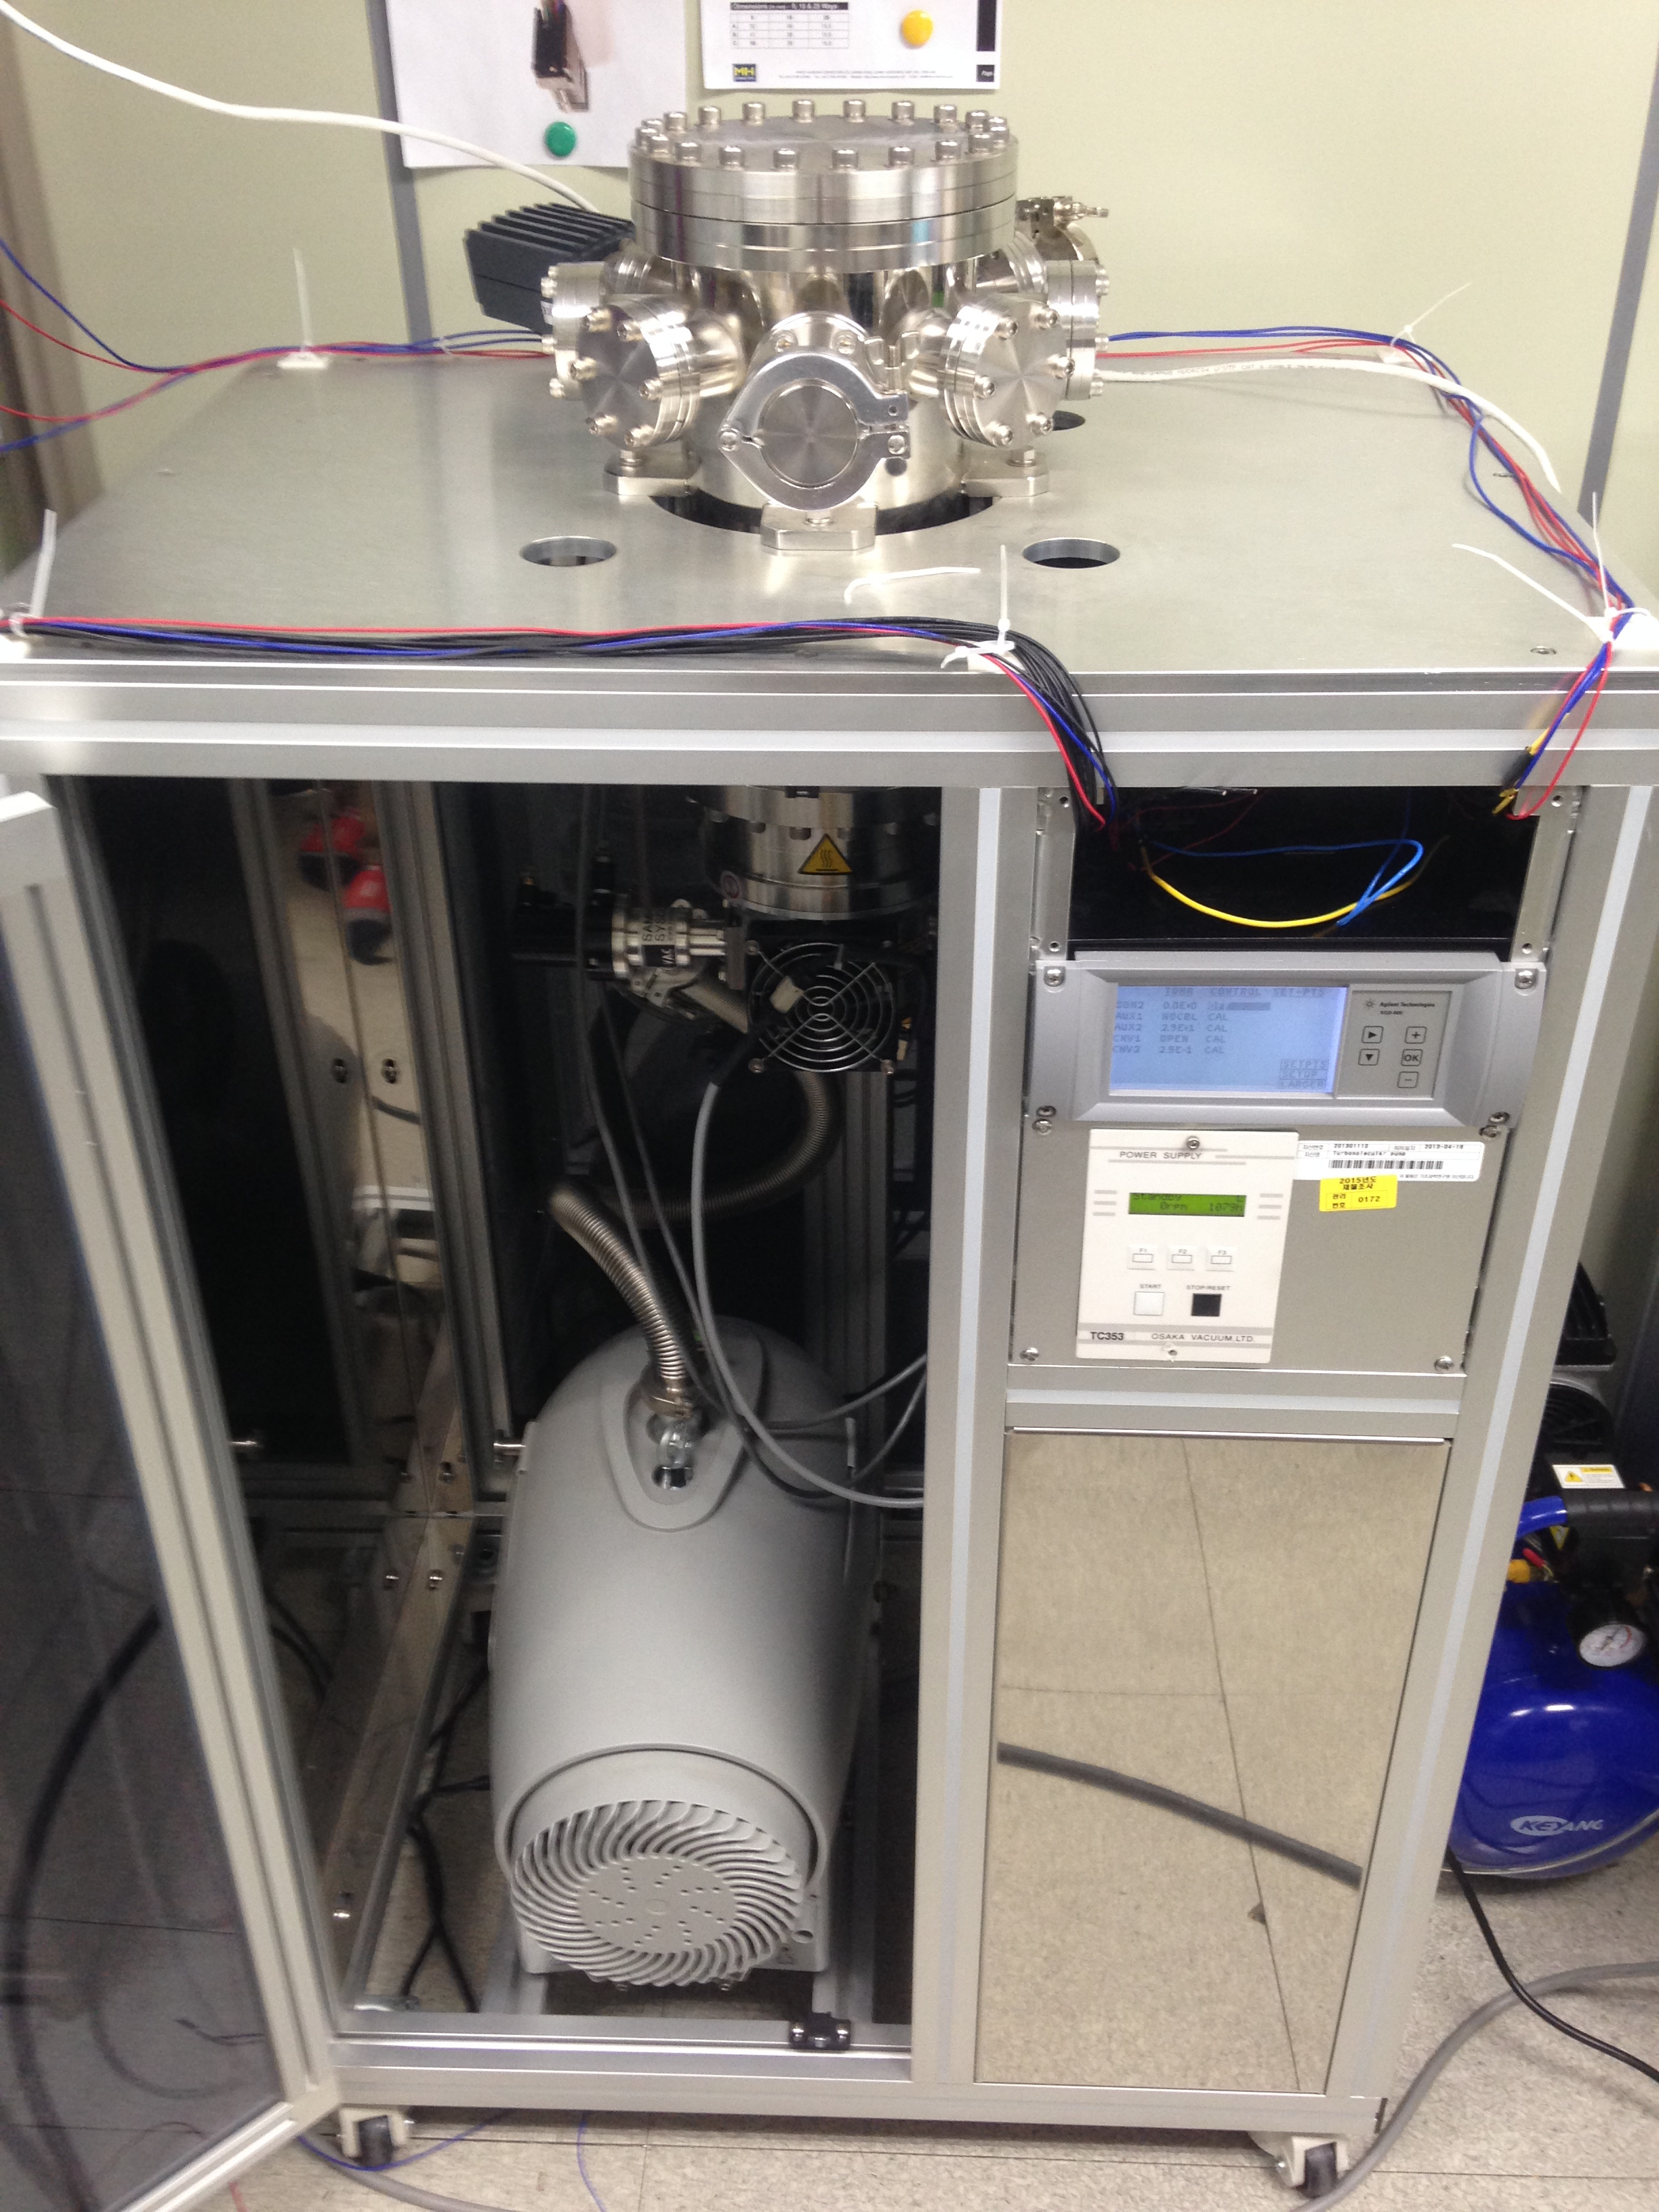
\includegraphics[width=1\columnwidth]{./images/vacuumsystem.eps}
\end{figure}
The Demo Vacuum Control system consists of below devices.

\begin{itemize}
    \item Turbo Molecilar pump (OSAKA TG450FCAB)\
	\item Gauge Controller (XGS-600) \& TMP controller (TC-353)\
	\item Convection gauge \& FKG-730 gauge\
	\item Gate valve \& Angle valve \
	\item Dry pump (IDP-15) \
\end{itemize}

\end{mdframed}

\section*{PLC module (Allen-Bradly)}
\begin{mdframed}[roundcorner=10pt]
	\vspace{2mm}
\begin{figure}[H]
	\centering
	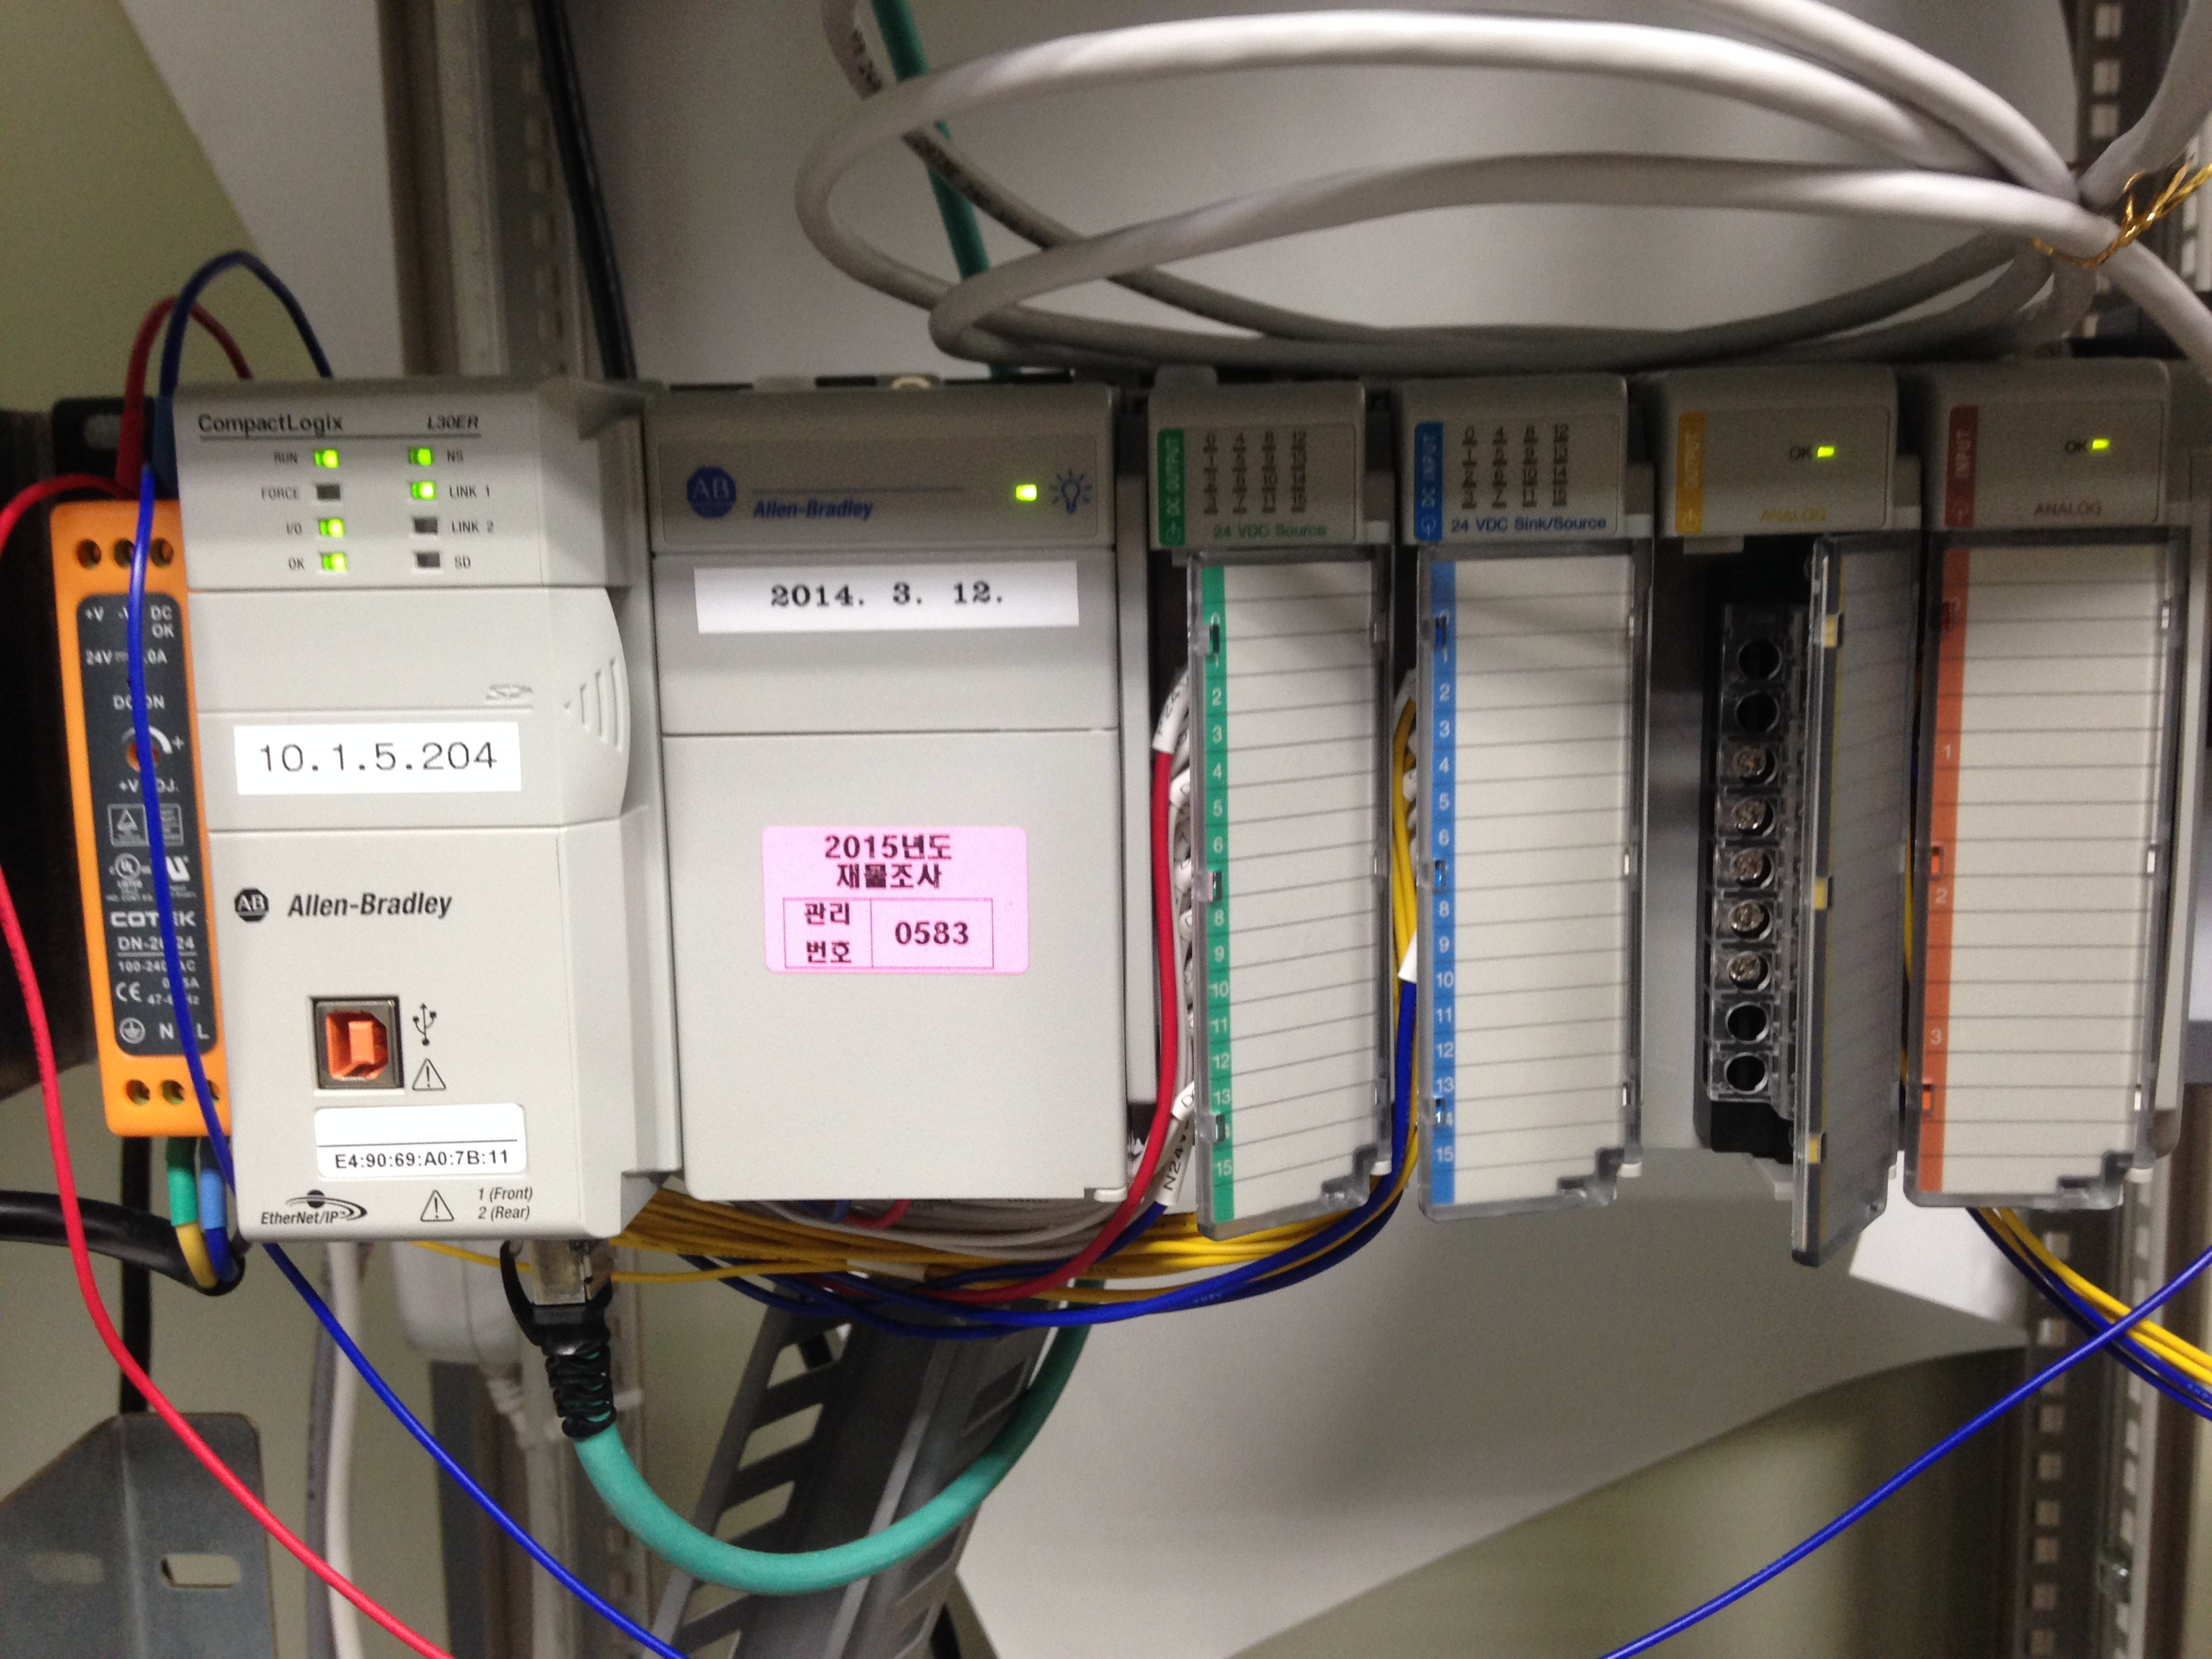
\includegraphics[width=1\columnwidth]{./images/compact.eps}
\end{figure}

Configuration of the PLC system

\begin{itemize}
	\item PLC CPU : L30ER
	\item Digital Input card : 1769-IQ16 (sink/Source)	
	\item Digital Output card : 1769-OB16
	\item Analog Input card : 1769-OF2
	\item Analog Output card : 1769-IF4
  	
\end{itemize}
\end{mdframed}

\columnbreak

\section*{Remote IO module}
\begin{mdframed}[roundcorner=10pt]
	\vspace{2mm}
	\begin{figure}[H]
		\centering
		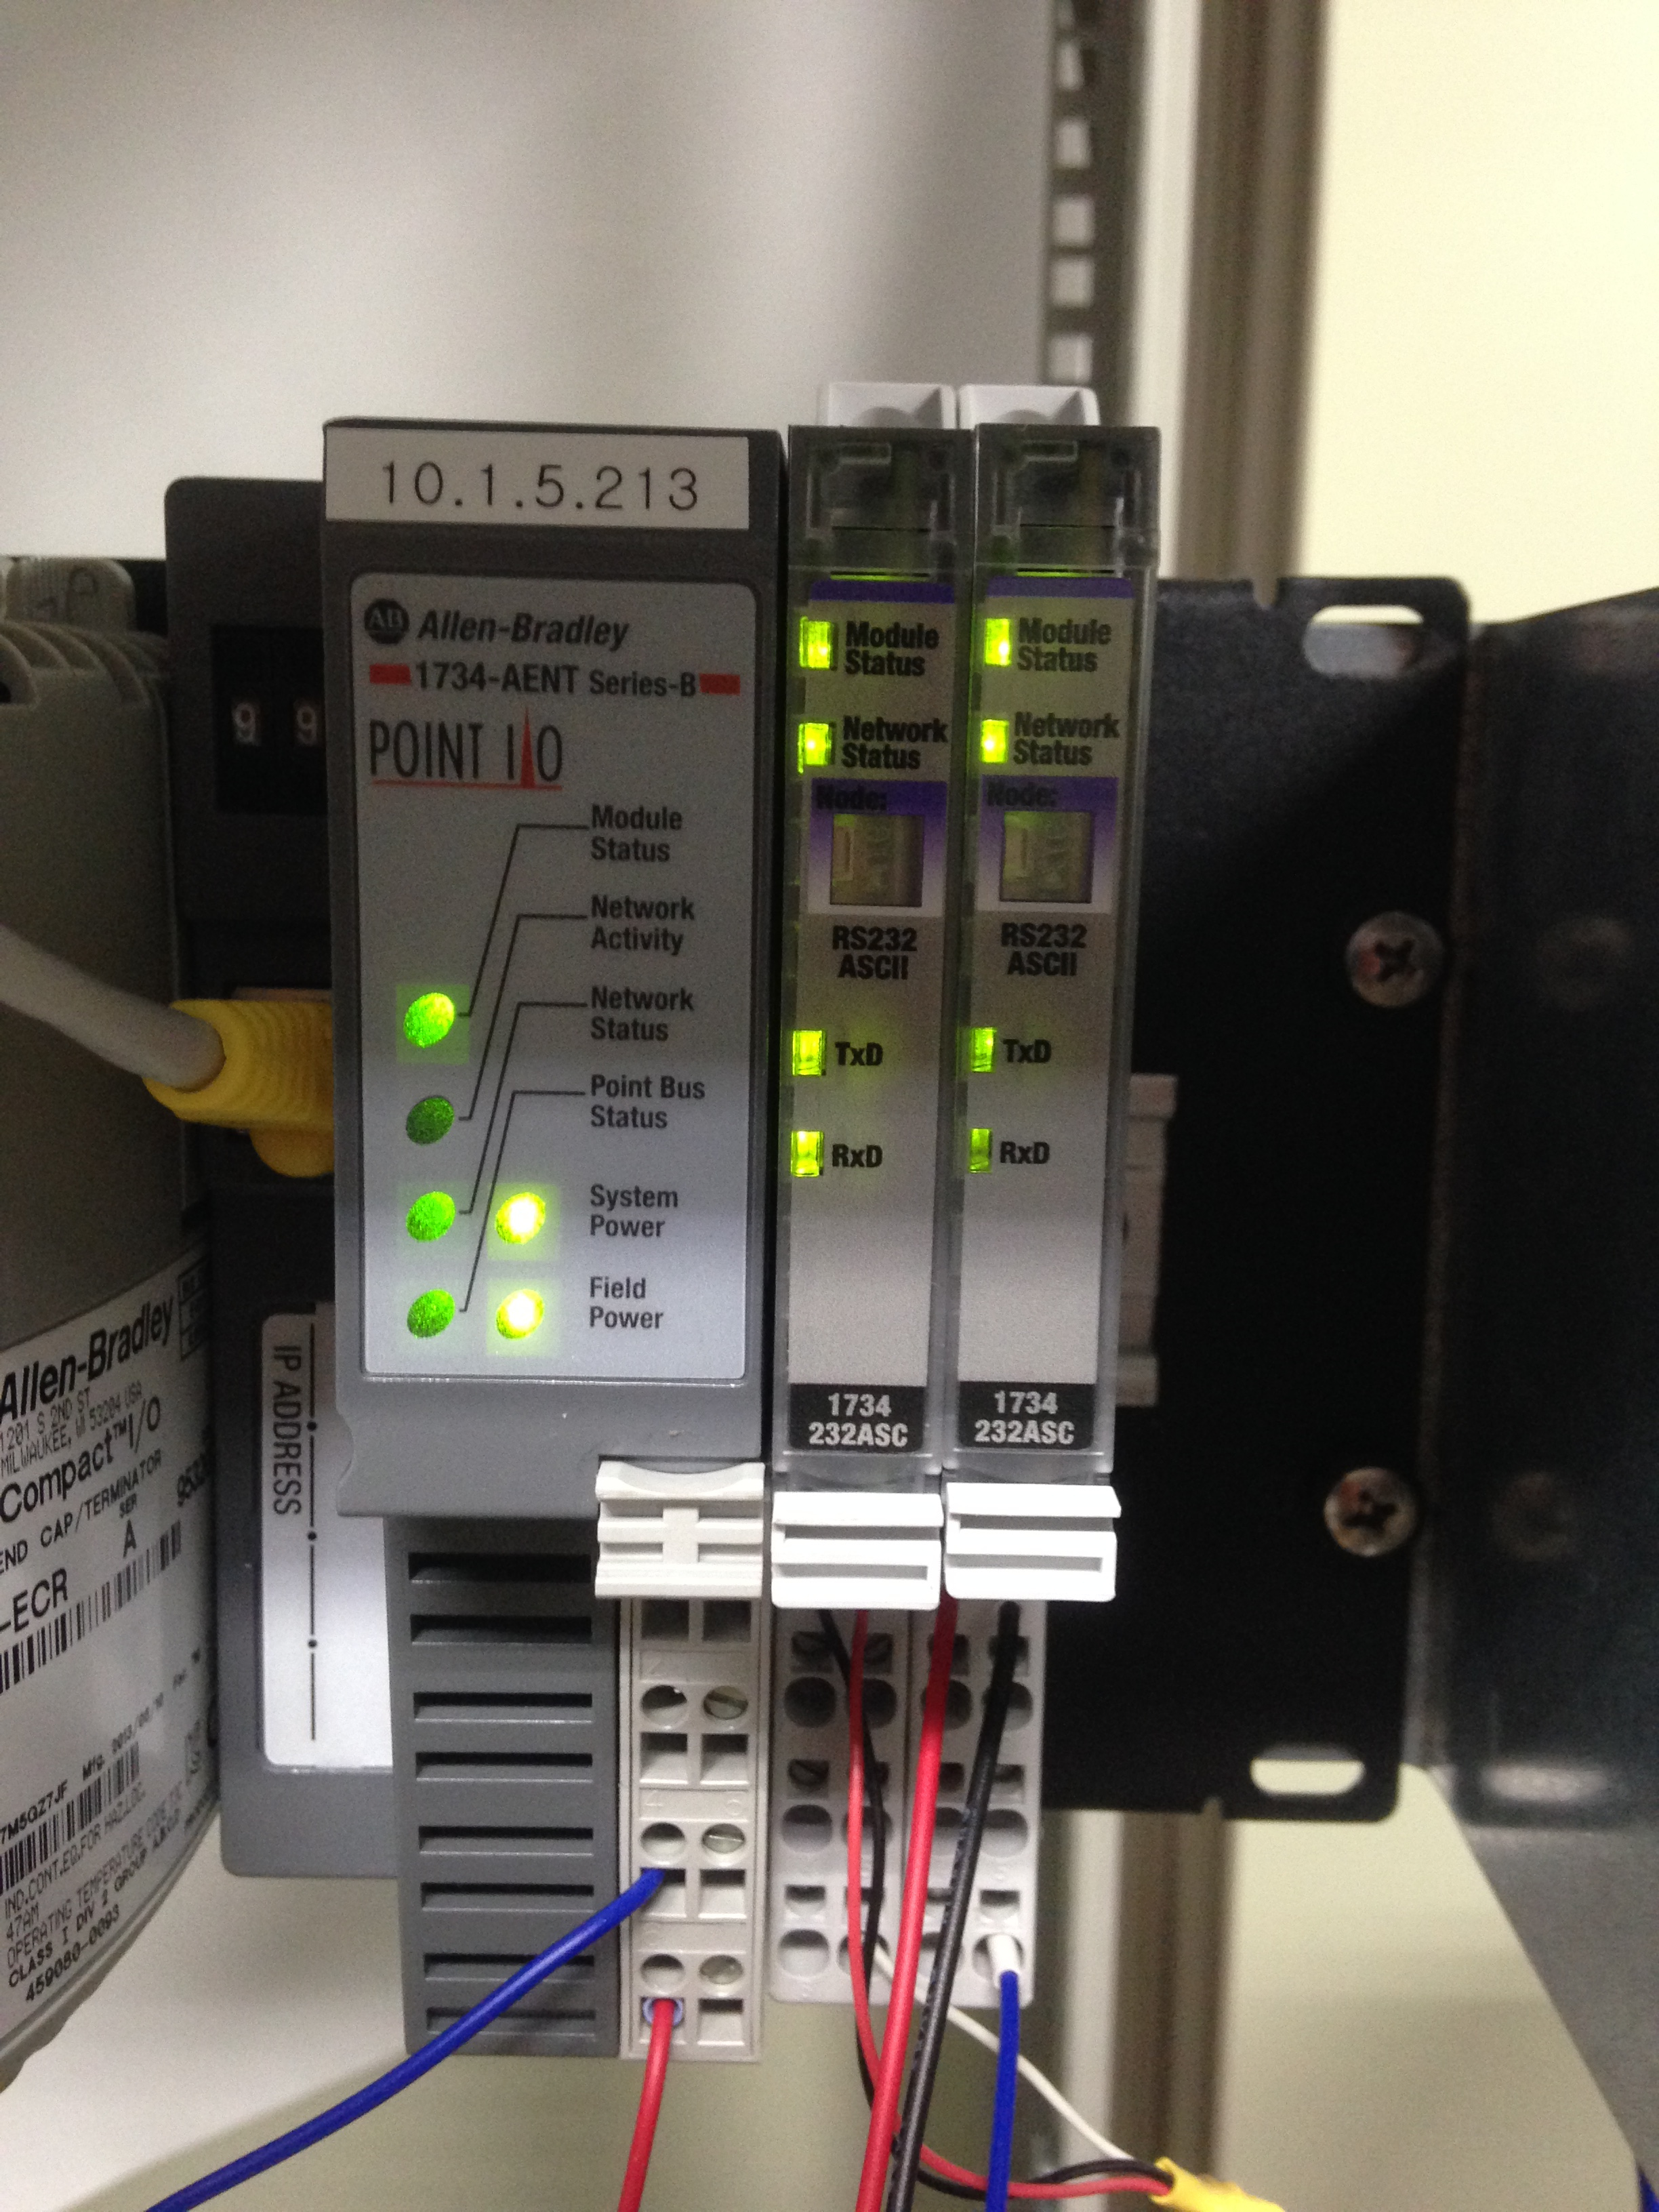
\includegraphics[width=0.7\columnwidth]{./images/pointIO.eps}
	\end{figure}
	
Serial communication modules are installed on remote module.

\begin{itemize}
	\item Remote IO module : 1734-AENT Point IO
	\item Serial communication card : 1734-232ASC, 2ea	
\end{itemize}
\end{mdframed}


\section*{Schematic of the control system}
\begin{mdframed}[roundcorner=10pt]
\begin{figure}[H]
  \centering
  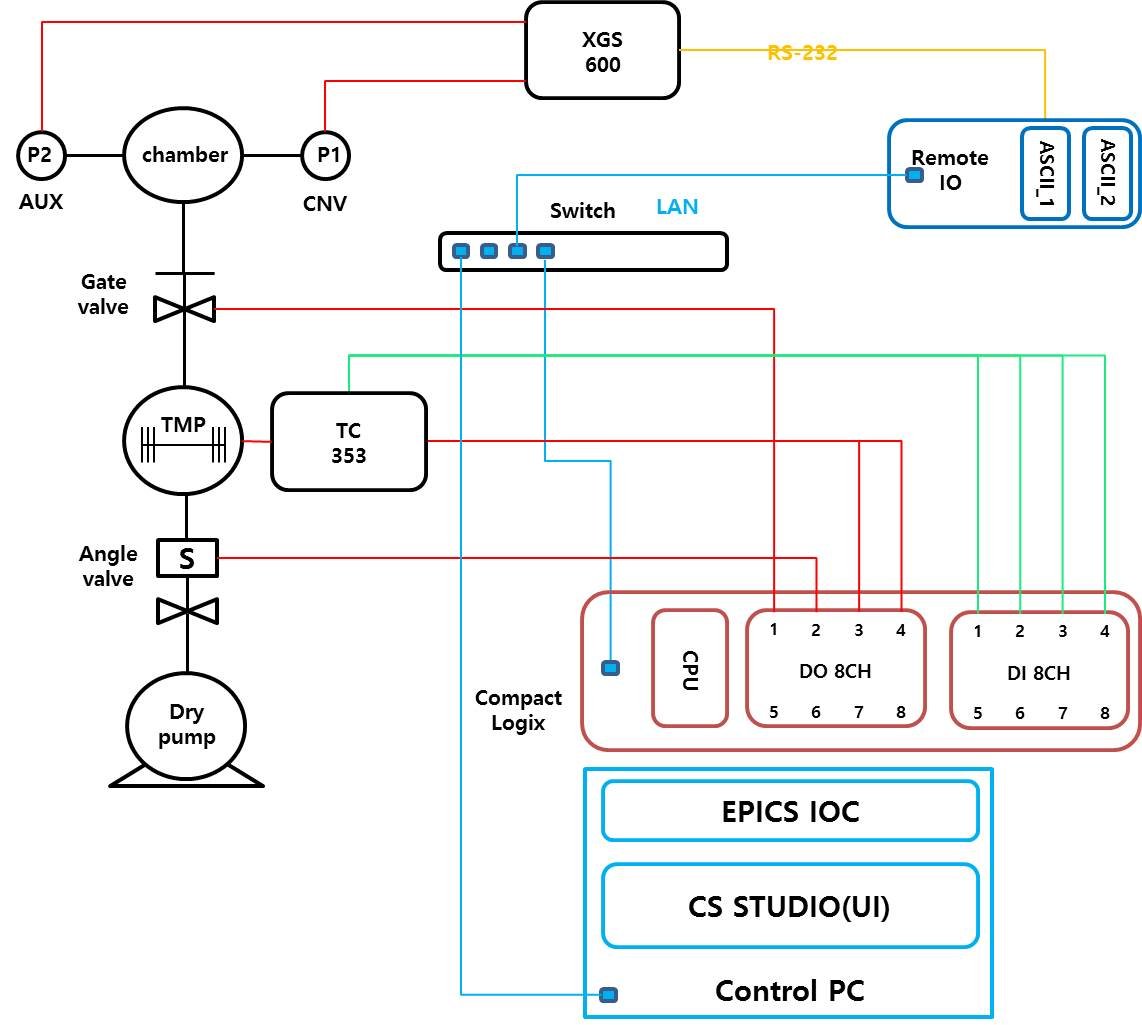
\includegraphics[width=1\columnwidth]{./images/configuration_diagram.eps}
  %\caption{Overall architecture of the RAON control system}
  \label{fig:architecture}
\end{figure}

\begin{itemize}
\item Vacuum devices are controlled by AB PLC \
\item RS-232 communication between PLC and XGS-600 \
\item RS-232 communication between PLC and TC-353 \
\item System monitoring by Control System Studio (CSS)\\
\end{itemize}
\end{mdframed}

\section*{PLC programing}

\begin{mdframed}[roundcorner=10pt]
\begin{figure}[H]
\centering
  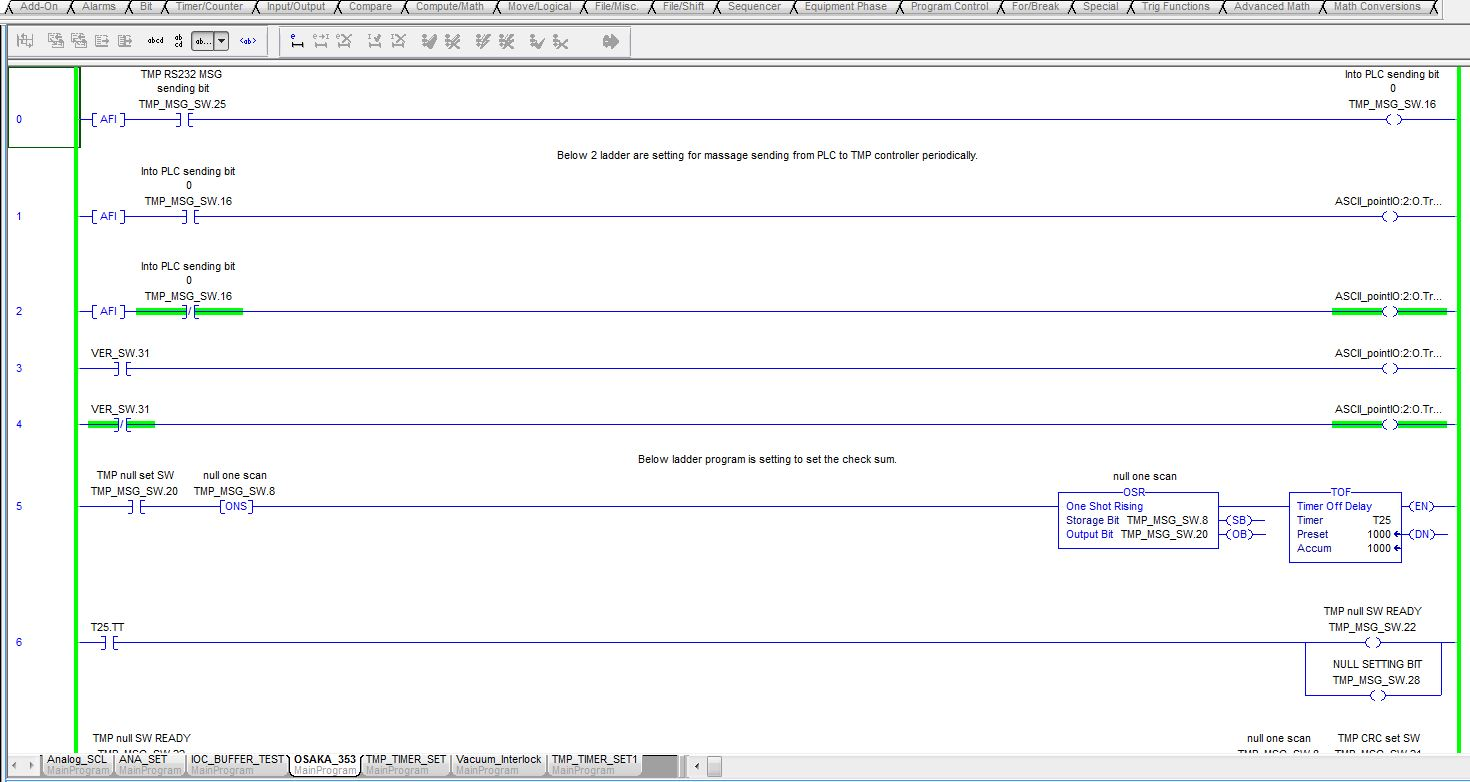
\includegraphics[width=0.96\columnwidth]{./images/PLC_LADDER.eps}
%\caption{The vacuum control system}
\label{fig:vacuum_control}
\end{figure}
\begin{figure}[H]
	\centering
	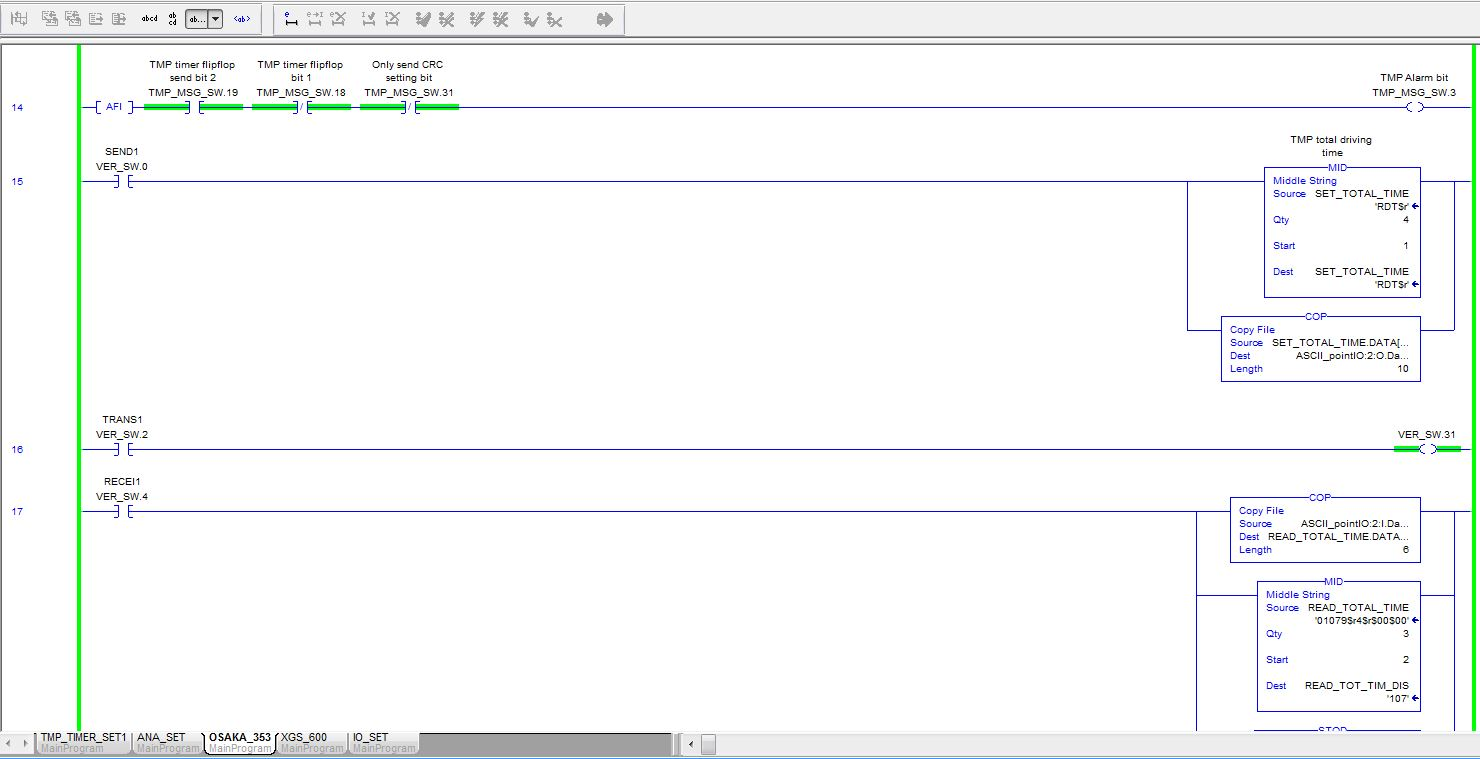
\includegraphics[width=0.96\columnwidth]{./images/Ladder1.eps}
	%\caption{The vacuum control system}
	\label{fig:vacuum_control}
\end{figure}


\begin{itemize}
\item PLC ladder program to control the all devices and to communicate with device controllers.
\end{itemize}
\end{mdframed}

\columnbreak


\section*{EPICS IOC configuration}

\begin{mdframed}[roundcorner=10pt]
	\begin{figure}[H]
		\centering
		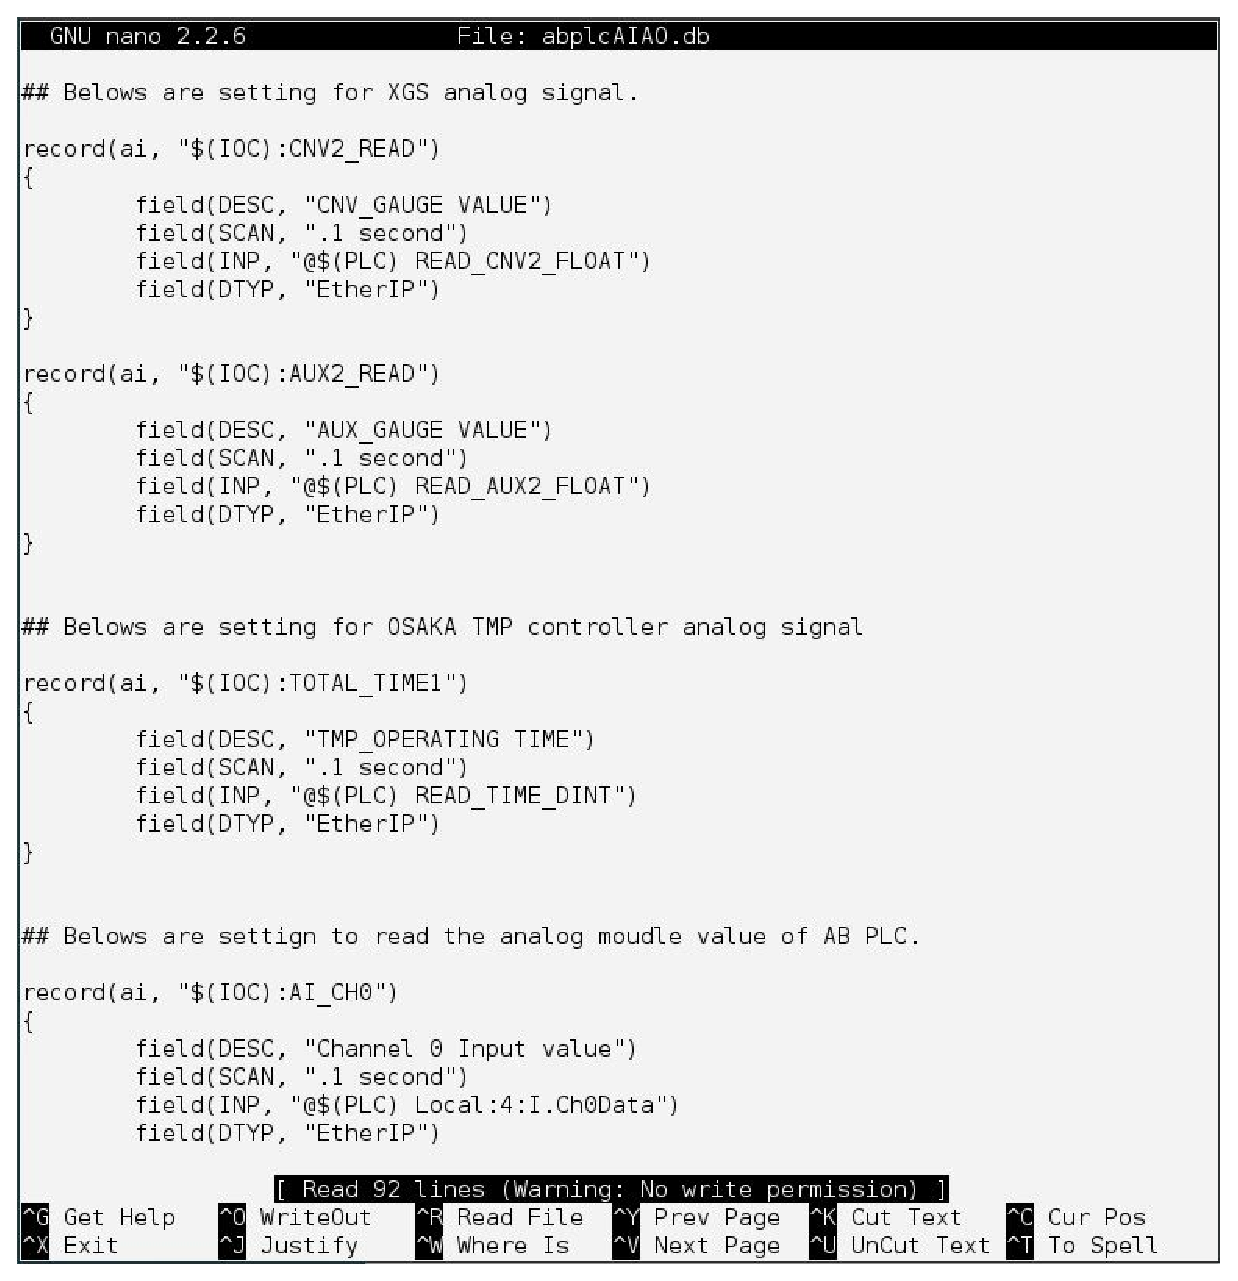
\includegraphics[width=1\columnwidth]{./images/db_file.eps}
		
	\end{figure}
	
	\begin{itemize}
		\item EPICS IOC database file configuration for matching address between PLC and EPICS PV.
	\end{itemize}
		
	\begin{figure}[H]
		\centering
		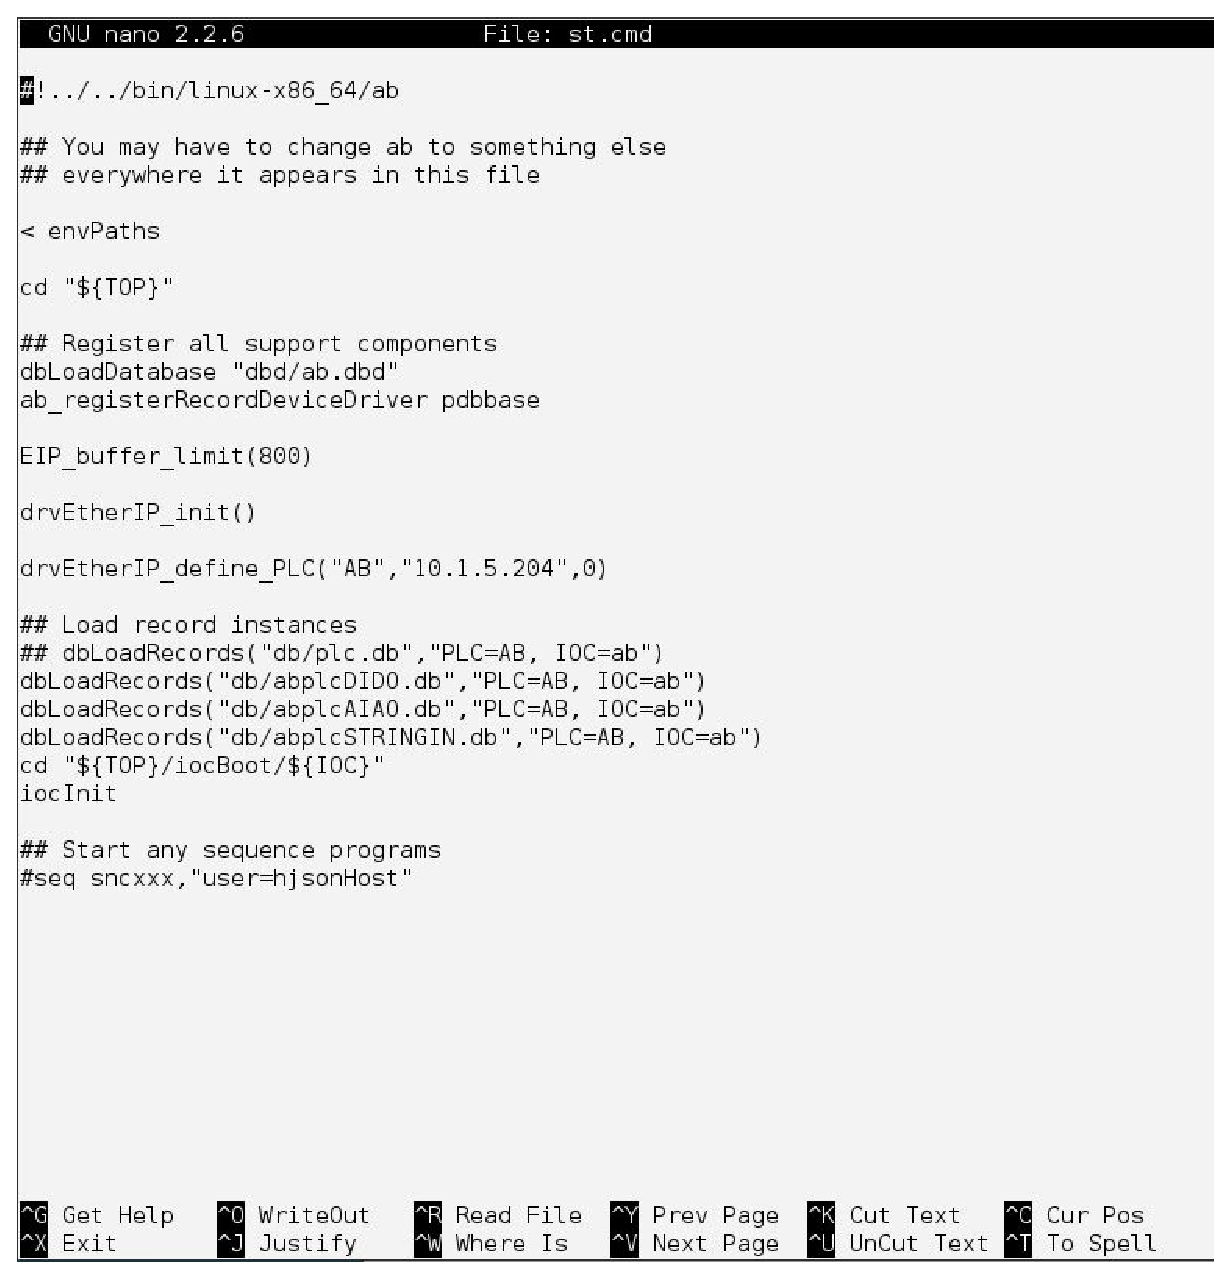
\includegraphics[width=1\columnwidth]{./images/stfile.eps}
	\end{figure}
		
	\begin{itemize}
		\item EPICS IOC command file configuration for environment setting to communicate with PLC.  
	\end{itemize}
	
In order to communicate between AB PLC and EPICS IOC, we used the ether-ip module which is released at EPICS homepage (http://www.aps.anl.gov/epics/).
	
\end{mdframed}

\section*{User Interface}
\begin{mdframed}[roundcorner=10pt]
	\vspace{2mm}
	\begin{figure}[H]
		\centering
		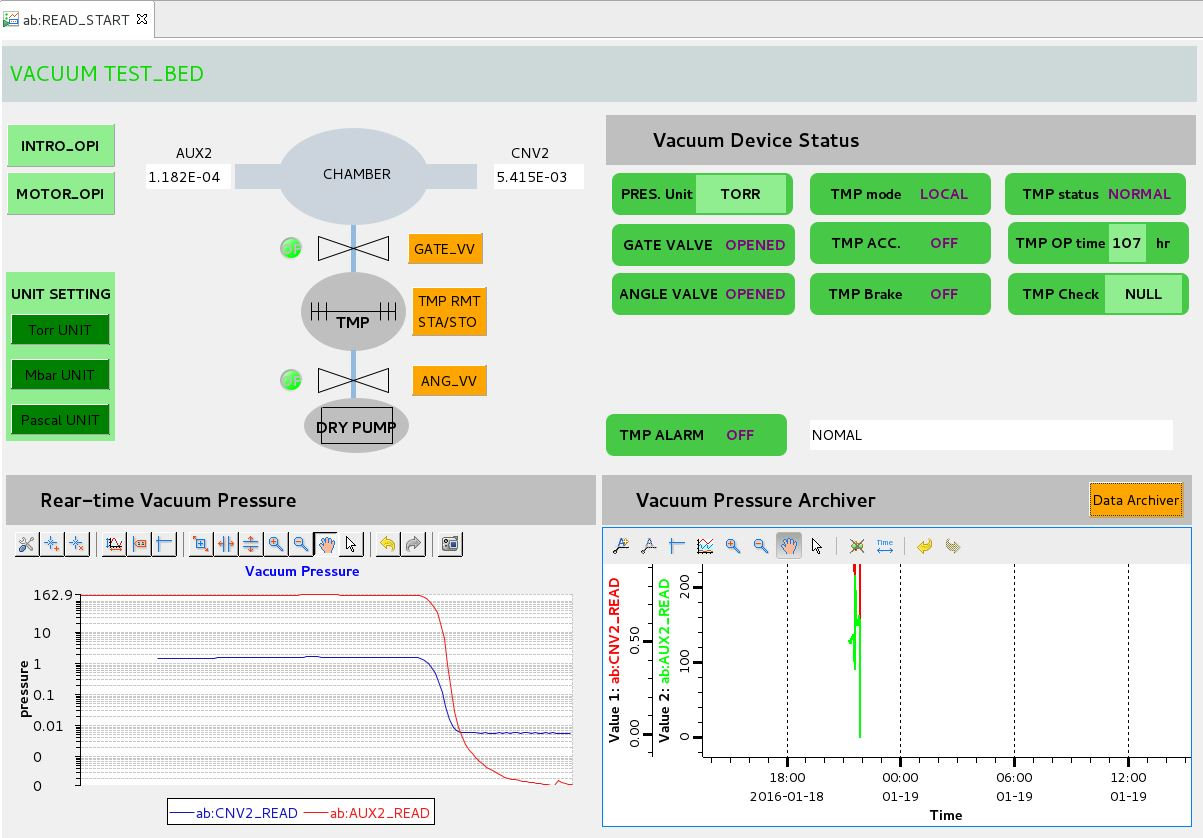
\includegraphics[width=1\columnwidth]{./images/UI1.eps}
	\end{figure}
	\begin{itemize}
		\item All pressure data could confirm on screen real-time.(lower left) 
		\item All data are archiving on local server in a form text file.(lower right)
	\end{itemize}
\end{mdframed}

\section*{Acknowledgement}
This work is supported by the Rare Isotope Science Project funded by Ministry of Science, ICT and Future Planning(MISP) and National Research Foundation(NRF) of Korea(Project No. 2011-0032011).

\end{multicols}

%\vspace{13mm}

%\begin{minipage}[b]{1\linewidth}

%\section*{RAON Major Operations Modes}
%\vspace{2mm}
%\begin{figure}[H]
 % \includegraphics[width=0.99\columnwidth]{./images/raon_all_modes.eps}
%\end{figure}

%\end{minipage}





\end{document}

